\documentclass[format=acmsmall, review=true, screen=true]{acmart}

\usepackage{syntax}
\usepackage{booktabs} % For formal tables
\usepackage{mathtools}
\usepackage{forest}
\usepackage{subcaption}
\usepackage[ruled]{algorithm2e} % For algorithms

\usepackage{tikz}
\renewcommand{\algorithmcfname}{ALGORITHM}
\SetAlFnt{\small}
\SetAlCapFnt{\small}
\SetAlCapNameFnt{\small}
\SetAlCapHSkip{0pt}
\IncMargin{-\parindent}


% Metadata Information
%\acmJournal{TWEB}
%\acmVolume{9}
%\acmNumber{4}
%\acmArticle{39}
%\acmYear{2010}
%\acmMonth{3}
%\copyrightyear{2009}
%\acmArticleSeq{9}

% Copyright
%\setcopyright{acmcopyright}
%\setcopyright{acmlicensed}
%\setcopyright{rightsretained}
%\setcopyright{usgov}
%\setcopyright{usgovmixed}
%\setcopyright{cagov}
%\setcopyright{cagovmixed}

% DOI
%\acmDOI{0000001.0000001}

% Paper history
%\received{February 2007}
%\received[revised]{March 2009}
%\received[accepted]{June 2009}

\usepackage{xcolor}
\newcommand\todo[1]{\textcolor{red}{#1}}

% Document starts
\begin{document}
% Title portion. Note the short title for running heads 
\title[Spineless]{Spineless Traversal for Layout Invalidation}  
\author{Marisa Kirisame {marisa@cs.utah.edu}}
\orcid{1234-5678-9012-3456}
\affiliation{%
  \institution{University of Utah}
  \streetaddress{201 Presidents' Cir, Salt Lake City, UT 84112}
  \city{Salt Lake City}
  \state{UT}
  \postcode{84112}
  \country{USA}}
\author{Tiezhi Wang {2152591@tongji.edu.cn}}
\orcid{1234-5678-9012-3456}
\affiliation{%
  \institution{Tongji University}
  \streetaddress{104 Jamestown Rd}
  \city{Williamsburg}
  \state{VA}
  \postcode{23185}
  \country{China}}
\author{Pavel Panchekha {pavpan@cs.utah.edu}}
  \orcid{1234-5678-9012-3456}
  \affiliation{%
  \institution{University of Utah}
  \streetaddress{201 Presidents' Cir, Salt Lake City, UT 84112}
  \city{Salt Lake City}
  \state{UT}
  \postcode{84112}
  \country{USA}}

\begin{abstract}

\end{abstract}

\newcommand{\DBPQpctslowdown}{0.23}
\newcommand{\DBPQpctspeedup}{0.77}
\newcommand{\DBPQoverhead}{3.27}
\newcommand{\DBPQeval}{1.01}
\newcommand{\DBPQtotal}{1.81}
\newcommand{\DBPQsmalloverhead}{5.96}
\newcommand{\DBPQsmalleval}{1.02}
\newcommand{\DBPQsmalltotal}{2.41}
\newcommand{\DBPQlargeoverhead}{1.29}
\newcommand{\DBPQlargeeval}{1.00}
\newcommand{\DBPQlargetotal}{1.17}
\newcommand{\TotalDiffCount}{4324}
\newcommand{\TotalTraceCount}{50}

\newcommand{\NumWebsites}{\TotalTraceCount}
\newcommand{\NumFrames}{\TotalTraceCount}
\newcommand{\MeanSpeedup}{\DBPQoverhead}
\newcommand{\MeanSpeedupSmall}{\DBPQsmalloverhead}
\newcommand{\PctSlower}{\DBPQpctslowdown}
\newcommand{\PctFaster}{\DBPQpctspeedup}

%
% The code below should be generated by the tool at
% http://dl.acm.org/ccs.cfm
% Please copy and paste the code instead of the example below. 
%
\begin{CCSXML}
<ccs2012>
 <concept>
  <concept_id>10010520.10010553.10010562</concept_id>
  <concept_desc>Computer systems organization~Embedded systems</concept_desc>
  <concept_significance>500</concept_significance>
 </concept>
 <concept>
  <concept_id>10010520.10010575.10010755</concept_id>
  <concept_desc>Computer systems organization~Redundancy</concept_desc>
  <concept_significance>300</concept_significance>
 </concept>
 <concept>
  <concept_id>10010520.10010553.10010554</concept_id>
  <concept_desc>Computer systems organization~Robotics</concept_desc>
  <concept_significance>100</concept_significance>
 </concept>
 <concept>
  <concept_id>10003033.10003083.10003095</concept_id>
  <concept_desc>Networks~Network reliability</concept_desc>
  <concept_significance>100</concept_significance>
 </concept>
</ccs2012>  
\end{CCSXML}

\ccsdesc[500]{Computer systems organization~Embedded systems}
\ccsdesc[300]{Computer systems organization~Redundancy}
\ccsdesc{Computer systems organization~Robotics}
\ccsdesc[100]{Networks~Network reliability}

%
% End generated code
%

% We no longer use \terms command
%\terms{Design, Algorithms, Performance}

\keywords{Web Browser, Incremental Computation, Algorithms, Performance}


\thanks{This work is supported by the National Science Foundation,
  under grant CNS-0435060, grant CCR-0325197 and grant EN-CS-0329609.

  Author's addresses: G. Zhou, Computer Science Department, College of
  William and Mary; Y. Wu {and} J. A. Stankovic, Computer Science
  Department, University of Virginia; T. Yan, Eaton Innovation Center;
  T. He, Computer Science Department, University of Minnesota; C.
  Huang, Google; T. F. Abdelzaher, (Current address) NASA Ames
  Research Center, Moffett Field, California 94035.}


\maketitle

% The default list of authors is too long for headers}
\renewcommand{\shortauthors}{M. Kirisame et al.}

\section{Introduction}

Latency is a major concern for modern web rendering engines
  such as those used in Chrome, Safari, and Firefox.
Ideally, a rendering engine
  would redraw the page 60 times per second
  to guarantee smooth animations, fluid interactions,
  and prompt responses as user browse and interact with web pages.
When this frame rate cannot be met,
  the user experiences lag, and may be forced to use another web application, browser, or device.
Moreover, demand for low-latency rendering is only increasing
  with modern 120\,Hz displays.

Layout is a key driver of web rendering latency.
Layout means calculating the size and position
  of each element of the web page,
  after which the page can be rendered into pixels on the screen.
Every time the user interacts with the web page
  by hovering over an element,
  receiving updated data,
  or even observing an animation,
  the web page, and thus its tree of nodes, changes.
To show the updated page to the user,
  the browser must then re-laid-out.
Since there are many rendering phases besides layout,
  layout must be completed in a sub-millisecond budget 
  n order to meet the 60 frame-per-second goal.
On such tight budget, every cycle counts!

\paragraph{Incrementalization}
The key optimization that makes this possible is \emph{incrementalization}. That is, when the web page changes, the browser identifies a subset of the page whose size and position can change. Specifically, the browser \emph{marks} all fields in all nodes that may need to be recomputed. Then, when the next frame must be drawn, the layout algorithm traverses the node tree to find and recompute those fields. For small layout changes---as one would see in an animation or interaction---traversing the tree to find those fields can be the bottleneck, especially since every node access is likely to incur an L2 cache miss.

The standard algorithm for finding and recomputing the dirty fields is a ``double dirty bit'' algorithm, which uses summary bits to avoid traversing unchanged subtrees of the node tree. While effective in many cases, this algorithm has a core flaw: it requires traversing the root node, every node between it and a dirty node, and any node adjacent to that path. This ``spine plus one'' can contain hundreds of clean nodes on large web pages, especially because web page node trees are typically far from balanced, often with both deeply-nested ``wrapper'' nodes and containers with dozens or hundreds of children. Since each node access introduces its own cache miss, traversing the ``spine plus one'' can stall the layout algorithm for hundreds of microseconds. Indeed, this problem had been widely observed. For example, Google's widely-used web performance debugging tool, Lighthouse, uses tree depth and maximum children count as performance metrics.

\paragraph{Spineless Traversal}

We introduce \textit{spineless traversal}: a new, faster algorithm for incremental layout. Unlike the standard ``double dirty-bit'' algorithm, spineless traversal accesses only dirty nodes, and therefore reduces cache misses. To do so, spineless traversal stores the set of invalidated nodes in a priority queue that allows jumping directly to the next dirty node. This avoids accessing the `+`spine plus one'' and thus achieves better latency.

The key to making this work is maintaining the correct traversal order. Recomputing a single field on a single node can ``dirty'' all fields that depend on it, and the set of transitive dependencies is complex. Fields must therefore be recomputed in a specific order, and spineless traversal must respect that order as it jumps from node to node. Spineless traversal enforces this using an \emph{order maintenance} data structure. Order maintenance assigns a logical time to each field on each node, and provides an efficient way to check which logical time comes first.

We implement spineless traversal in a new DSL for browser layout algorithms, Megatron. To match the extremely-tight latency budgets of modern browsers, Megatron uses a variety of low-level optimizations, including unboxing, a custom allocator, pointer compression, and a five-cycle instruction sequence for logical time comparisons.

\paragraph{Evaluation}
As our main test case, we implement a fragment of the CSS~2.1 specification in Megatron. Our fragment includes complex features including line breaking, flex-box, \texttt{display} changes, intrinsic sizes, min/max width/height, and absolute positioning and is based on the Cassius~\cite{cassius-1} formalization of CSS~2.1. Our implementation of this fragment covers over 700 lines and involves computing approximately 50 properties for every node. This implementation provides a realistic and taxing workload for invalidation algorithms.

We execute this implementation, using both the standard double dirty bit algorithm and the spineless traversal algorithm, on  \TotalDiffCount incremental layouts of \TotalTraceCount real-world web pages, including Twitter, Discord, Github, and Lichess. Spineless Traversal is \DBPQoverhead times as fast on average. On small changes, which typically represent interactions like hover, typing, or animations, spineless traversal achieves speedups of \todo{$10\times$} or more. Meanwhile, the largest layout invalidations, which typically are less-latency-critical events like page loads, only see a slowdown of \todo{$30\%$}, with only \todo{$30\%$} of incremental layouts seeing a slowdown.


\section{Web layout}

Web page source code is written in HTML,
  which is a tree-structured markup language
  containing text and elements that wrap it.
The web browser's parsed representation of this tree
  is called the DOM tree.
To draw the page to the screen,
  the browser applies a sequence of transformations---%
  rendering phases---%
  to this DOM tree: matching, styling, layout, paint, and so on.
The focus of this paper, the layout phase,
  applies to an intermediate tree structure
  called a ``layout tree'',
  whose shape largely matches the DOM tree,
  though with some deviations.
The layout phase reads properties from layout tree nodes
  (which reflect HTML attributes, CSS properties, and other data)
  and computes layout fields like width and height for those nodes.
Later phases like paint then read those layout fields
  and use them to draw the page to the screen.
In memory,
  the layout tree is stored as a pointer tree,
  with the children stores as a doubly linked list.
This is necessary for fast insertions and deletions,
  but also means that layout nodes are
  often spread throughout memory,
  with every access generating a cache miss.


\begin{figure}
\scalebox{0.7}{
\begin{forest}
  [body 
    [header [a] [div [nav [a] [a] [a] [a] [a]] [nav [a]]]]
    [div 
      [ol 
        [li 
          [div 
            [div [a] [div]] 
            [div 
              [span [a]] 
              [span [a] [a]]
              [a]
              [div 
                [a [img]] 
                [span]
                [a]
                [span]
                [span]
                [span [input] [label [div [a] [a] [a]]]] 
                [span [span] [a]]]]]]
        [a [span]]]
    [div]
    [ol
      [li
        [div
          [form
            [input]
            [input]
            [input
              [div
                [textarea
                  [p]
                  [div
                    [input] [button] [div]]]]
              [p]]]]]
      [li]]]
    [footer [a] [a] [a] [a]]
    [span]]
\end{forest}
}
\centering
\caption{A dom tree representation
  of a page on \texttt{lobste.rs},
  an online forum / news aggregator,
  with just a single link and no comments.
Text nodes are not shown.
The page nonetheless contains 69 elements,
  with the maximum width of 7 and maximum depth of 10;
  in other words, the page is highly imabalanced.
Among the links (\texttt{<a>} elements),
  the spine+1 can contain as many as 30 elements, half the complete tree,
  due to the unbalanced tree.}
% https://lobste.rs/s/7ixd88/c_complexity_compiler_bugs
\label{fig:dom-tree-raw}
\end{figure}

\subsection{The Layout Phase}

Computing layout fields is a recursive process
  because each node's layout depends on the layout of its neighbors.
For example, the height of a node is (typically)
  the sum of the heights of all its children,
  while a node's $x$ position depends on the $x$ position
  of its previous sibling, plus that previous sibling's width.%
\footnote{
  In reality, these rules are quite a bit more complex,
    with various exceptions to the simplified sketch given here.}
Moreover, visible properties like width and height
  in turn depend on intermediate properties such as intrinsic size,
  current line width/height, and more obscure properties
  like the sum of its siblings' \texttt{flex-grow} values.
A complete layout pass must visit each node multiple times,
  in a well-defined order,
  in order to compute each field on each node
  before any others that depend on it.

\begin{figure}
\begin{verbatim}
def layout_simple(self): # real layout much more complex
  for c in self.children:
    layout_simple(c)
  self.height <-
    if has_path(last) then last.height_acc 
    else self.attribute[height]
  self.height_acc <-
    if has_path(prev) then prev.height_acc + self.height 
    else 0
\end{verbatim}
\caption{A layout algorithm that compute width of each dom node. The above program is a tree traversal: it walk down the tree then walk up the tree, computing values for each node during the walk.}
\label{fig:layout-simple}
\end{figure}

\iffalse
\begin{figure}
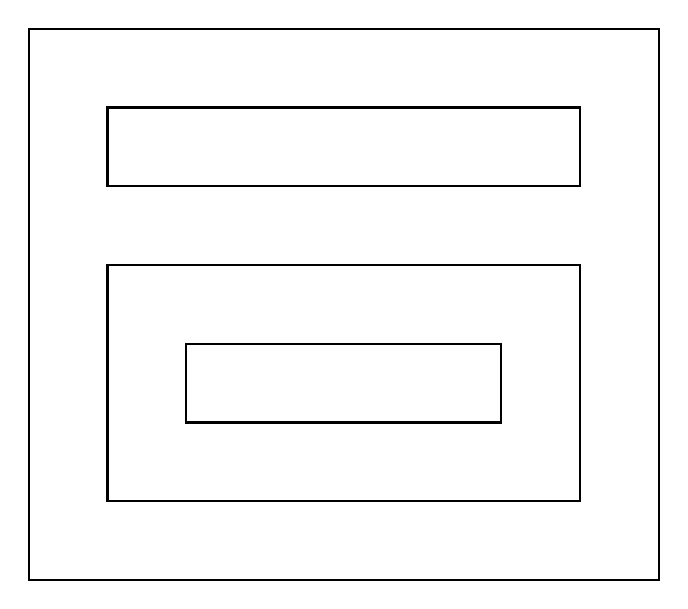
\begin{tikzpicture}
\draw[black, thick] (0,7) rectangle (8,0);
\draw[black, thick] (1,6) rectangle (7,5);
\draw[black, thick] (1,4) rectangle (7,1);
\draw[black, thick] (2,3) rectangle (6,2);
\end{tikzpicture}
\caption{The HTML document is laid-out into multiple boxes, forming a tree.}
\end{figure}
\fi

\begin{figure}
\centering
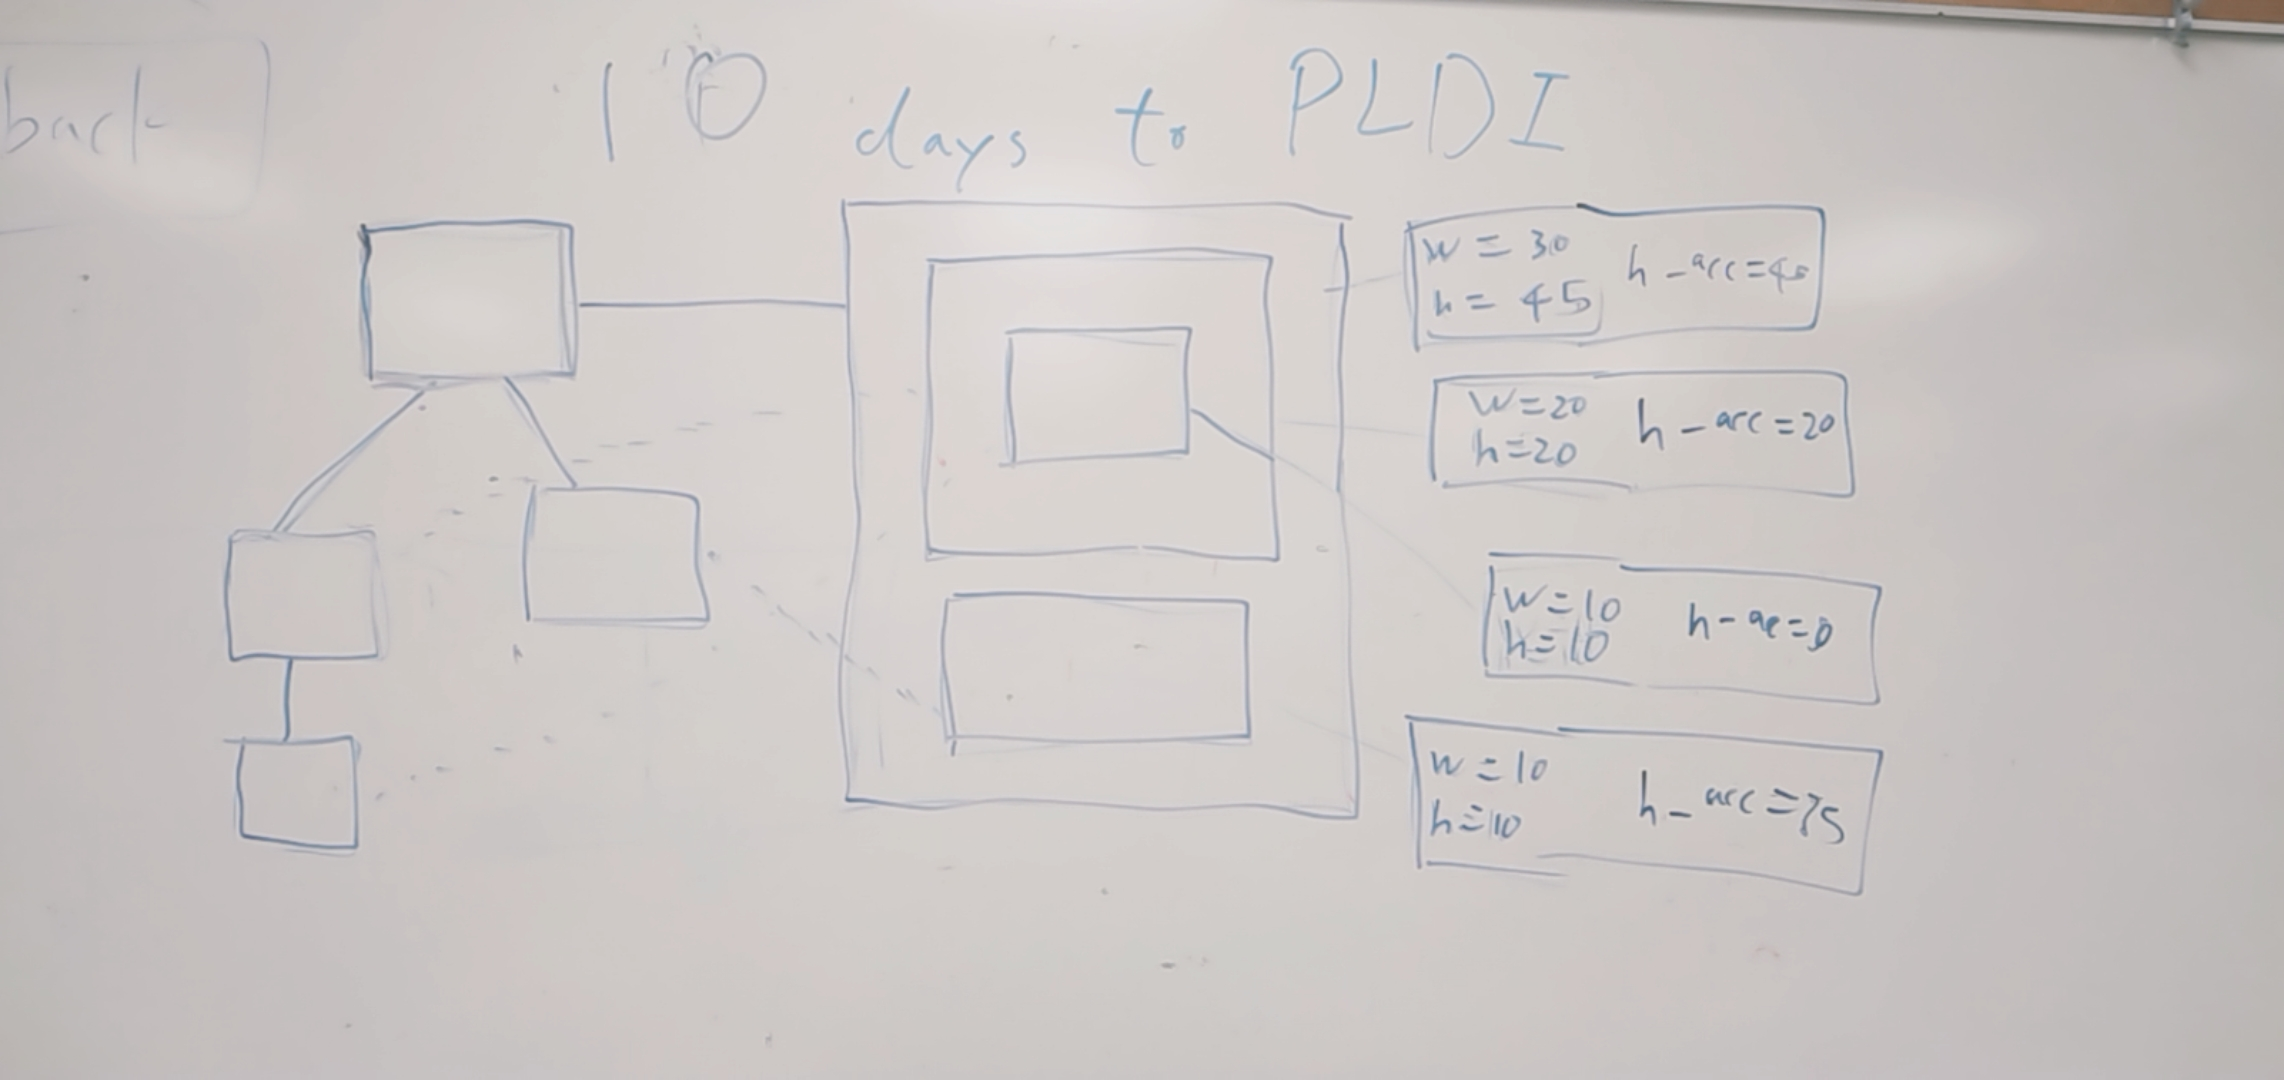
\includegraphics[scale=0.15]{layout.jpg}
\caption{A tree, its property, and the box model}
\end{figure}

We remark on a couple of key properties of layout
  that influence our approach:
\begin{enumerate}
    \item{Bounded work}: a fixed, bounded amount of work is performed per node. There are no data-dependent loops, recursions, or data structures except over the layout tree itself.
    \item{Immutable shape}: the layout tree itself is not modified during layout; only the computed fields on each node are. Moreover, these computed fields are only written once (per frame) and then become read-only (for that frame).
    \item{Static control flow}: the fields are computed in a fixed order dependent only on the layout tree shape, not the values of other computed fields.
    \item{Local data flow}: to compute a particular node's fields, only that node's neighbors in the layout tree and their fields are accessed.
\end{enumerate}
In other words, layout can be expressed in the DSL
  shown in Figure~\ref{fig:dsl}.

In this DSL, a layout is defined by a set of passes
  $\text{Pass}_n$ performed in a certain order (the schedule).
Each pass performs a recursive, in-order traversal of the tree,
  computing some fields pre-order and some fields post-order.
Computing a field just requires
  a simple assignment $\mathsf{self}.V \gets T$,
  where $V$ is a computed field on the current node $\mathsf{self}$
  and $T$ is an expression that can refer to
  other fields on $\mathsf{self}$ and its neighbors
  $\mathsf{parent}$, $\mathsf{prev}$, $\mathsf{next}$,
  $\mathsf{first}$ (child), and $\mathsf{last}$ (child).
Computations can also refer to HTML attributes or CSS properties
  of the DOM node corresponding to the current layout node
  using $\mathsf{attribute}[x]$ or $\mathsf{property}[x]$.%
\footnote{
    We use two different namespaces
    for HTML attributes and CSS properties
    because some names, like \texttt{height},
    appear in both sets.
    There's a special property for the tag name.
    The exact details differ between browsers
    but do not affect spineless traversal,
    so we ignore the distinctions here.
}
Expressions can also use conditionals
  to test whether a given neighbor exists ($\mathsf{N?}$).
The DSL is more flexible than it may at first appear:
  for example, if a node wants to access a field on its grandparent,
  instead of accessing $\mathsf{parent}.\mathsf{parent}.\mathsf{x}$,
  each node could define a $\mathsf{parent\_x}$ field which copies
  its parent's $x$ value,
  and then access $\mathsf{parent}.\mathsf{parent\_x}$.
In any case, prior work in similar DSLs%
  ~\cite{meyerovich-1, meyerovich-2, cassius-1,
  cassius-2, cassius-3, yufeng-1, yufeng-2}
  has already shown that layout features
  like the CSS box model, \texttt{display: none},
  absolute positioning, flexible box layout,
  and line breaking are expressible in such a language.

A key property of a layout $L$
  is the order in which it computes
  different fields on different nodes in the tree.
Specifically, let the \emph{trace} of a layout on a tree $T$
  be sequence of $(n, v)$ pairs
  where $n$ is a node in $T$ and $v$ is a field name in $L$.
Because our DSL only performs in-order traversals,
  the trace is structurally related to the tree shape:
  local changes to the tree (node insertions or deletions)
  imply local change to the trace (subtrace insertion or deletion).
This structural relation means
  that the ordering of any two $(n, v)$ pairs is fixed:
  if $(n, v)$ appears before $(n', v')$,
  this appear-before relationship
  will be maintained even as new nodes are added or removed.% 
\footnote{
  We assume here that
    only brand-new nodes, not previously-removed ones,
    are inserted into the tree.
  To our knowledge, this assumption is true
    of all major web rendering engines.
}

In the remainder of this paper,
  we will assume a correct implementation
  of web page layout exists in this DSL,
  with correctness meaning both the correct set of rules
  and also a correct schedule for computing them
  while preserving dependencies.
Our own implementation (Section~\ref{sec:layout-impl})
  implements a subset of widely-used web layout features;
  however, spineless traversal is applicable
  to any layout expressed in this DSL,
  and we do not focus on the details
  of the rules or schedule further.
Notably, our DSL enforces
  the key properties of layout described above:
  there is no functionality to mutate the tree shape
  or to reorder control flow according to field values.
There are also no loops or data structures,
  and the only field access allowed is to a node's neighbors.

\begin{figure}

\begin{align*}
\text{Layout} &\coloneq  \{\:
  \mathsf{rules}: \text{Rule}^+,
  \mathsf{schedule}: \text{Pass}_n^+
\:\} \\
\text{Rule} &\coloneq
  \mathbf{def}\:\text{Pass}_n()\:\{\:
    A^+;\:
    \mathsf{children}.\mathsf{forEach}(\text{Pass}_n);\:
    A^+;\:
  \} \\
A \in \text{Assignment} &\coloneq
  \text{self}.V \leftarrow T \\[4pt]
T \in \text{Term} &\coloneq
  \text{if}\ T\ \text{then}\ T\ \text{else}\ T \mid
  F(T^+) \mid
  N? \mid
  N.V \mid
  \mathsf{attribute}[V] \mid
  \mathsf{property}[V] \\
N \in \text{Neighbor} &\coloneq
  \mathsf{self} \mid \mathsf{prev} \mid
  \mathsf{next} \mid \mathsf{parent} \mid
  \mathsf{first} \mid \mathsf{last} \\[4pt]
V \in \text{Variable} &\coloneq \text{unique symbols} \quad\quad
F \in \text{Function} \coloneq \text{primitive functions}
\end{align*}
\caption{
  A minimal DSL for defining web layout
    as a set (\textsf{rules}) of passes
    performed in a specific order (\textsf{schedule}).
  The syntax $P^+$ represents a sequence of non-terminal $P$.
  Passes are in-order traversals of the layout tree
    performing a sequence of assignments to local fields
    while accessing fields of the current node or its neighbors.
}
\label{fig:dsl}
\end{figure}


\subsection{Incremental layout}

Layout needs to be performed any time
  a user interaction or JavaScript code
  modifies the DOM tree,
  typically in response to a user interaction like
  clicks, hovers, drags, animations, or typing.
The DOM tree modification
  can change the value of an HTML attribute or CSS property
  (as happens when the user selects a drop-down item
  or types into a text box)
  or it can insert and delete nodes in the DOM
  (as might happen when a page is loaded or new content
  is inserted from the network),
  but most of these modifications,
  and especially the most latency-critical,
  like hovers, drags, animations, and text editing,
  modify only a small portion of the DOM tree at a time
In either case,
  once the DOM node changes,
  the layout tree must change as well.
If DOM nodes are added or removed,
  layout nodes typically must be as well;
  layout nodes can also be removed
  by modifying some HTML attribute (like \texttt{hidden})
  or CSS properties (like \texttt{display: none}).
Then, whether or not DOM nodes are added or removed,
  the computed value of various layout fields
  may change and need to be recomputed.

In order to achieve this,
  each layout node maintains a \textit{dirty} bit for each field,
  which defines whether that field value needs to be recomputed.%
\footnote{In a real browser, often one boolean bit
  summarizes whether any in a set of fields need to be recomputed,
  but we describe a bit per field here for simplicity.}
The dirty bit is set when a layout node is added to the tree,
  and is cleared when its associated field is computed.
A field is also dirtied when a value it depends on changes.
For example, in the simple layout of Figure~\ref{fig:layout-simple},
  when a node's \texttt{height} attribute is changed,
  its \texttt{height} field is marked dirty.
Then, when that \texttt{height} field is recomputed,
  its \texttt{height\_acc} field can in turn be marked dirty.
When the \texttt{height\_acc} field is recomputed,
  its next sibling's \texttt{height\_acc} field is then marked dirty.
Alternatively, if a node is deleted,
  the \texttt{height} of its parent
  (if it was the last child)
  and the \texttt{height\_acc} of its next sibling
  must be marked dirty.

However, recomputing a field does not mark any dependent fields
  if the newly-computed value matches the previous value.
This optimization is critical:
  it means that many changes affect only a
  small fraction of the layout tree,
  since their effects are localized to a subset of it.
For example, you might imagine that typing into a multi-line text box
  can move around the text within the text box
  but, if the text box has a fixed height,
  won't affect the size or position of anything outside it.
In other words, fields are marked dirty when
  HTML attributes or CSS properties change,
  or when nodes are added and removed from the DOM;
  then these dirty bits propagate through the layout tree
  until all affected nodes are marked and recomputed.%
\footnote{
  As described this is a flow-insensitive dependency analysis;
    it is possible to do a finer-grained flow-sensitive analysis instead.
  This design decision is orthogonal to the algorithms presented in this paper.
}

Importantly, dirty bit propagation code
  can be synthesized from the layout algorithm.
To do so, one analyzes every assignment $\mathsf{self}.V \gets T$
  in the layout program.
For each field access $N.U$ in the expression $T$,
  we know that $\mathsf{self}.V$ depends on $N.U$,
  meaning that any changes to $\mathsf{self}.U$
  must mark $N^{-1}.V$ as dirty,
  where $N^{-1}$ is the inverse of the relation $N$;
  flipping \textsf{next} and \textsf{previous},
  mapping \textsf{first} and \textsf{last} to \textsf{parent},
  and mapping \textsf{parent} to all children.
Note that, if the original algorithm respects the dependency order,
  then a field is only computed after all fields that it depends on.
This in turn means that, after a field is computed,
  it can no longer be marked dirty.
This guarantees termination:
  computing a field clears its dirty bit, so by the end of an incremental layout
  every field is clean.

Insertion and deletion require particular care
  in propagating dirty bits.
An inserted node has all of its new fields marked dirty;
  likewise, deleting a node marks all dependants of its fields.
Inserting or deleting nodes can also change
  $\mathsf{N?}$ expressions;
  any fields that use such expressions must then
  also be marked dirty.%
\footnote{Once again,
  this could use a flow-sensitive analysis or a simpler
  flow-insensitive one.
The invalidation challenges are similar in either case.}
Importantly, an entire subtree can be inserted or deleted at once;
  this is quite common in real-world web pages
  where pop-ups or menus can appear as a result of a hover or click.
Since all data accesses in our model are local,
  only the root of the subtree actually needs to be considered,
  meaning that deleting or inserting a subtree takes constant time,
  regardless of the size of the subtree.

\subsection{Recomputation}
With the dirty bit marking algorithm mentioned above, 
  the problem of incremental layout is now reduced to 
  finding all dirtied fields, and recomputing them, 
  in the dependency order.

A naive incremental implementation can recursively traverse 
  the tree as if rerunning from scratch, 
  but only re-assign value to the dirtied node. 
This trivial invalidation algorithm nonetheless
  respects the dependency order and clears all dirtied fields.
It also recomputes only dirtied fields,
  performing a minimal number of recomputations.
However, since it traverses the entire tree,
  in incurs just as many cache misses as a non-incremental layout
  and therefore does not lead to a significant speed-up.
Driven by this observation, we can immediately classify
  accessed nodes into two types: the dirtied nodes,
  which have fields dirtied and must be accessed to
  recompute them, and the auxiliary nodes, 
  which does not have fields dirtied, but are nonetheless 
  accessed in order to find and reach the dirtied node.
The number of dirtied nodes is set by
  the dependency structure of web layout,
  but the number of auxiliary nodes can be reduced
  through better algorithms for finding dirtied nodes.

\subsection{Double Dirty Bit}
The SOTA algorithm,
  which we dub the Double Dirty Bit algorithm,
  achieves this by adding a second dirty bit
  per pass, which indicates whether
  any field assigned during pass
  is dirty in the \emph{subtree} rooted at a node.
This summary bit is initially off, and when a node is marked,
  the summary bit is turned on.
Since the summary bit is recursive over the subtree,
  setting a summary bit must also set the parent's summary bit,
  stopping at the root node
  or at a node with the summary bit already on.

\begin{figure}
\begin{verbatim}
def find_dirty_nodes(self):
    if self.dirty:
        yield self
    if self.summary_bit:
        # Access spine + 1
        for child in self.children:
            find_dirty_nodes(child)
\end{verbatim}
\caption{Finding the dirty nodes in a tree.}
\label{fig:find-dirty-nodes}
\end{figure}

The summary bit allows layout to skip recursing into a subtree
  when the summary bit is off.
An example implementation, conceived as an iterator
  that yields dirty nodes,
  is shown in Figure~\ref{fig:find-dirty-bits}.
The Double Dirty Bit algorithm
  greatly reduces the number of nodes accessed,
  improving performance,
  and is considered the state of the art
  for layout invalidation~\cite{tali-garseil,wbe}.

However, the Double Dirty Bit algorithm
  nonetheless accesses a number of auxiliary nodes.
To reach any dirty node,
  the Double Dirty Bit traversal must
  must traverse the path from the root of the tree
  to the dirtied node---the ``spine'' of that node.
Moreover, each node along that spine
  will have its summary bit set,
  meaning that the Double Dirty Bit algorithm will recurse
  into that node's children.
In other words,
  the Double Dirty Bit algorithm has, as its auxiliary nodes,
  both the spine of each dirtied node,
  and also all children of that spine.
Since web layout trees have both very wide and very deep nodes,
  this can be a very large set of auxiliary nodes.
For example, the \texttt{lobste.rs} web page
  shown in Figure~\ref{fig:dom-tree-raw}
  has an \texttt{<input>} element at depth 8,
  which represents a dropdown that a user might interact with.
An interaction like opening and closing the dropdown
  will affect only a few elements
  (likely seven:
    the \texttt{<input>},
    its sibling \texttt{<label>},
    and its parent \texttt{<span>}),
  but its spine contains eight nodes
  and adding the children of the spine nodes
  brings the total number of auxiliary nodes to 22.
If (oversimplifying) cache misses are the only cost,
  Double Dirty Bit would have then have
  $22 / 7 \approx 3\times$ overhead for this interaction,
  unnecessarily increasing latency.

Unsurprisingly, these auxiliary nodes
  are a significant source of latency,
  affecting both browser and web developers.
Google Chrome's Lighthouse performance monitoring tool~\cite{lighthouse},
  for example, warns if tree depth or fanout is high.
This implicitly means that achieving the expected performance,
  especially on a highly-interactive web application
  such as Figma, VS Code, Office 365, or Photoshop,
  may require changing the global shape of the layout tree.
Naturally, an invalidation algorithm that simply
  did not require so many auxiliary nodes
  would be a superior solution.

\begin{figure}
\scalebox{0.7}{
\begin{forest}
  [body 
    [header [a] [div [nav [a] [a] [a] [a] [a]] [nav [a]]]]
    [div 
      [ol 
        [li 
          [div 
            [div [a] [div]] 
            [div 
              [span [a]] 
              [span [a] [a]]
              [a]
              [div 
                [a [img]] 
                [span]
                [a]
                [span]
                [span]
                [span [input] [label [div [a,color=blue] [a, color=green, for ancestors={color=red, for siblings={color=blue}}, name=CurrentDirtied] [a, color=orange, name=NextDirtied]]]]
                {\draw[->,dotted] (CurrentDirtied)--(NextDirtied);}
                [span [span] [a]]]]]]
        [a [span]]]
    [div]
    [ol
      [li
        [div
          [form
            [input, color=blue]
            [input, color=yellow, for ancestors={color=red, for siblings={color=blue}}]
            [input, color=blue,
              [div
                [textarea
                  [p]
                  [div
                    [input] [button] [div]]]]
              [p]]]]]
      [li]]]
    [footer [a] [a] [a] [a]]
    [span]]
\end{forest}
}
\centering
\caption{The Double Dirty Bit algorithm in action. The green "a" is the dirtied node, with the spine marked red, and the siblings of the spine marked blue, forming the spine+1. We assume the green "a" dirtied its next sibling, the orange "a". Note that the subsequent marking only dirty nodes on the spine+1, or their children, so maintaining summary bits and finding subsequent dirty node is quick. Other node (in this case, the yellow 'input' element) might also be dirtied, and the spine is reused.}
% https://lobste.rs/s/7ixd88/c_complexity_compiler_bugs
\label{fig:dom-tree-db}
\end{figure}
\section{Spineless Traversal}

Spineless Traversal improves on Double Dirty Bit
  by jumping directly between dirty nodes
  without accessing any auxiliary nodes;
  as a result, it suffers dramatically fewer cache misses.
Achieving this requires a more computationally heavy approach:
  storing all dirty nodes in a priority queue
  and maintaining the correct traversal order
  using an order maintenance data structure.
Spineless Traversal's savings in cache misses
  typically outweigh the greater computational requirements
  of these data structures.
Since Spineless Traversal is complex,
  this section develops it incrementally,
  first introducing the idea of a queue storing dirty nodes,
  then adding timestamps to maintain traversal order,
  and finally introducing the order maintenance structure
  to handle node insertion and deletion.
A final step optimizes bulk insertions and deletions.

\subsection{Jumping Directly to Dirty Nodes}

To jump directly to dirty nodes,
  we introduce a queue
  that stores pointers to dirty nodes.
More specifically, elements of the queue represent
  dirty bits in the layout tree that need to be cleared,
  and are represented in the queue by
  a pointer to the relevant layout node
  and an enumeration identifying
  which dirty bit needs to be cleared.
When a dirty bit is set,
  the corresponding node and enumeration are added to the queue;
  the order of nodes in the queue will be explained later.
Note that dirty bits are still present on layout nodes;
  elements are only added to the queue
  when a dirty bit is set for the first time,
  so the queue does not contain duplicates.
To perform an incremental layout,
  elements are popped from the queue
  and the relevant fields on the relevant node are recomputed,
  and clearing the relevant dirty bit.
In the process, new dirty bits may be set,
  so new elements may be added to the queue.
This is repeated until the queue is empty.
Only dirty nodes are ever in the queue,
  meaning only they---not auxiliary nodes---are ever accessed.

Concretely, the queue is stored in a packed array,
  meaning that clearing a dirty bit accesses
  one dirty element,
  plus its at most five neighbors.
If the queue stays in L2 cache due to repeated access,
  while elements do not due to their size,
  this means clearing a dirty bit incurs
  a maximum of six L2 cache misses---%
  much fewer than the number of auxiliary accesses
  typical of Double Dirty Bit.

\subsection{Maintaining Queue Order}

To ensure that each field is only recomputed once,
  queue elements must be in the right order.
We thus add a timestamp field
  for every dirty bit on every node,
  giving timestamps the same relative order
  as in a from-scratch layout.
In the full Spineless Traversal algorithm,
  as explained below,
  this timestamp is an ``order maintenance object'',
  but for now the reader can imagine it an integer counting up from 0.
The queue of dirty nodes is then refined to a priority queue,
  ordered by these timestamps.
The priority queue ``pops'' the element with the lowest timestamp,
  thus ensuring that Spineless Traversal clears dirty bits
  in timestamp order and thus clears each dirty bit exactly once.

Concretely, we use a min-heap as our priority queue,
  which is cache-friendly and requires
  relatively few operations for each push and pop.
Timestamps are stored adjacent to dirty bits,
  meaning they do not introduce any new L2 cache misses.
The priority queue is typically small:
  while there are typically thousands of nodes,
  with each node having dozens of fields in our evaluation,
  the priority queue typically contains less than 1000 elements,
  and for the most latency-critical interactions,
  like hovers or drags, it can contain 100 or fewer.
With such a small size, a priority queue push/pop requires
  5--10 timestamp comparisons,
  which can be performed in roughly the time
  of one to three L2 cache misses
  in our optimized implementation.

\subsection{Order Maintenance}

The final challenge is efficiently assigning timestamps
  to every dirty bit on every node.
Simple incrementing integer timestamps, sadly,
  don't work when nodes are inserted or deleted:
  inserting a node would shift all future timestamps,
  so while inserting the node and performing incremental layout
  might access only a few nodes,
  reassigning timestamps would access many more.
Instead, following SAC~\cite{SAC},
  Spineless Traversal uses
  an \emph{order maintenance} data structure (OM)
  to assign timestamps.
First introduced by \citet{OM},
  order maintenance is a data structure
  that maintains a totally ordered set of objects
  while allowing objects
  to be added and removed from the order arbitrarily.
Crucially, adding, removing, and comparing nodes takes $O(1)$ time.
Abstractly, order maintenance provides the following API:

\begin{enumerate}
\setlength{\itemindent}{8em}
  
\item[$\mathsf{Compare}(p, q)$] Decides whether $p$ or $q$ comes first in the order (or are equal).
\item[$\mathsf{Head}()$] Returns the first object of the order.
\item[$\mathsf{Create}(p)$] Creates and returns a new object right after $p$.
\end{enumerate}

\noindent
Deleting OM objects is also possible, though by default
  our implementation does not do so.%
\footnote{On long-running pages this is a memory leak,
  albeit a very slow one;
  enabling OM object deletion adds
  only a minor slowdown to Spineless Traversal,
  roughly 2\%.}

Our implementation is based on that by \citet{SOM},
  which uses a two-level structure with
  a double-linked list of double-linked lists.
Objects are represented by nodes in the lower-level lists.
Both levels are ordered;
  the total order traverses lower-level lists in order,
  in the order dictated by the higher-level list.
Each object (node in the lower-level list)
  maintains a pointer to its higher-level list cell;
  two objects are in the same low-level list
  if they have the same higher-level pointer.
To allow fast comparisons between nodes,
  both low-level and high-level list cells store
  an unsigned integer of fixed size
  (in our implementation, 32~bits)
  called labels.
Within both lists, node labels are strictly increasing;
  this makes comparisons fast.
Specifically, comparison has two cases:
  if the two objects are in the same low-level list,
  their labels are compared directly,
  while if they are in in different ones,
  their parents' labels are compared.
This comparison operation is
  the bulk of the Spineless Traversal time
  so its speed is essential;
  \Cref{sec:opt} discusses critical micro-optimizations
  that bring its latency down to around 5~cycles.

To create an object inside an order maintenance structure,
  a new lower-level list cell is created
  whose label is the average of the two neighboring labels.%
\footnote{
  When creating a node after the last node,
  the maximum representable number is used as the larger number.
}
If the two labels differ by exactly 1, however,
  this would repeat a label.
In this case, the data structure re-balances itself,
  evenly reassigning labels to existing objects.
This process might
  create a new higher-level list cell
  to split a lower-level list in two,
  ensuring a sufficiently large gap between its cells.
Rebalancing is algorithmically tricky
  but is not a significant time sink in our use case,
  so we do not detail re-balancing here;
  details can be found in \citet{SOM}.

\begin{figure}
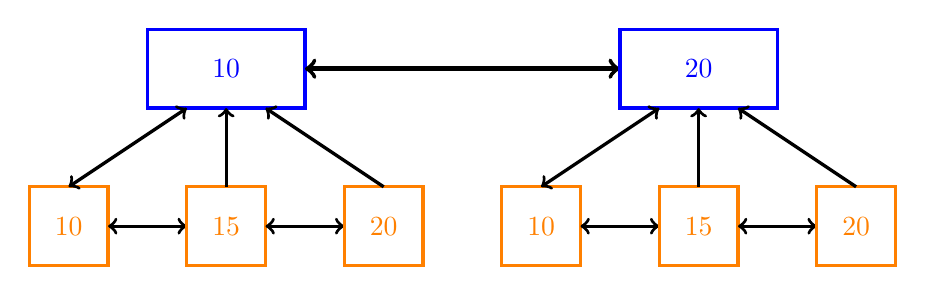
\begin{tikzpicture}
\draw[blue, very thick] (1.5,0) rectangle (3.5,1) node[pos=.5]{10};
\draw[ultra thick, <->] (3.5,0.5) -- (7.5,0.5);
\draw[blue, very thick] (7.5,0) rectangle (9.5,1) node[pos=.5]{20};

\draw[orange, very thick] (0, -2) rectangle (1,-1) node[pos=.5]{10};
\draw[very thick, <->] (0.5,-1) -- (2,0);
\draw[very thick, <->] (1,-1.5) -- (2,-1.5);
\draw[orange, very thick] (2, -2) rectangle (3,-1) node[pos=.5]{15};
\draw[very thick, ->] (2.5,-1) -- (2.5,0);
\draw[very thick, <->] (3,-1.5) -- (4,-1.5);
\draw[orange, very thick] (4, -2) rectangle (5,-1) node[pos=.5]{20};
\draw[very thick, ->] (4.5,-1) -- (3,0);

\draw[orange, very thick] (6, -2) rectangle (7,-1) node[pos=.5]{10};
\draw[very thick, <->] (6.5,-1) -- (8,0);
\draw[very thick, <->] (7,-1.5) -- (8,-1.5);
\draw[orange, very thick] (8,-2) rectangle (9,-1) node[pos=.5]{15};
\draw[very thick, ->] (8.5,-1) -- (8.5,0);
\draw[very thick, <->] (9,-1.5) -- (10,-1.5);
\draw[orange, very thick] (10, -2) rectangle (11,-1) node[pos=.5]{20};
\draw[very thick, ->] (10.5,-1) -- (9,0);

\end{tikzpicture}
\caption{An Order Maintenance data structure. The blue node represent the higher level doubly linked list, and each node store a lower level doubly linked list, denoted by the orange node. Lower level node also store a pointer to the higher level node. Each node additionally hold an unsigned integer, label, such that inside a single list the node earlier have a strictly smaller label then the node later.}
\label{fig:om}
\end{figure}

Concretely, the timestamp for each dirty bit
  is now represented by a pointer to the lower-level OM object.
Priority queue elements are a node pointer,
  an enumeration naming the dirty bit,
  and a pointer to the OM node,
  padded to a total of 16 bytes to align with cache lines.
To compare two timestamps, both pointers must be dereferenced
  to access the two lower-level OM objects.
The associated higher-level OM objects must also be accessed.
In the typical case, where the priority queue remains small,
  all of these OM objects in the priority queue
  are already in cache,
  so ``pops'' have no additional cache misses,
  while ``pushes'' add one, for the new element OM cell.
In total, all the priority queue and order maintenance operations
  thus add the equivalent of 3--5~L2~cache misses in latency,
  about 100--200 cycles.
Since recomputing a field, accessing neighbors' fields,
  and setting neighbors' dirty bits can itself take hundreds of cycles,
  Spineless Traversal's overhead is fairly small.

\subsection{Subtree Insertion}
\label{sec:tree-insertion}

Bulk insertions into the layout tree
  are common in ``lazy loading'' patterns:
  a ``shell'' web page loads first and shows a loading indicator;
  then the ``content'' loads and is inserted a large subtree,
  replacing the loading indicator.
This pattern is encouraged by frameworks like React,
  and can occur in several stages, with a ``shell''
  first inserting ``subshells'' which
  themselves load subcomponents in turn.
Efficiently handling these bulk insertions
  requires special care in Spineless Traversal,
  as bulk insertions are typically responsible
  for Spineless Traversal's worst performance
  relative to Double Dirty Bit.

The basic issue is that in a fresh subtree being inserted into the page,
  every field needs to be computed
  and every OM object needs to be initialized,
  without causing the priority queue itself to grow large.
Our solution adds these ``initialization passes''
  as special elements in the priority queue:
  besides $(v, n)$ pairs for a dirty field $v$ on node $n$,
  an element can also be $(p, r)$,
  a pass $p$ that needs to initialize the entire subtree rooted at $r$.
The timestamp for such a special element
  is just after the last field assigned by $p$
  in $T$'s previous sibling or parent.%
\footnote{
  An edge case is inserting a subtree into
    a subtree that itself has not yet been laid out.
  In this case no further actions need to be taken,
    since both subtrees will be visited together.}

When one of these $(p, r)$ elements is popped from the queue,
  the pass $p$ is performed on the whole subtree under $r$,
  creating all necessary order maintenance nodes
  and computing all fields assigned by $p$.
Since all data accesses are local,
  no existing nodes will refer to any newly-inserted node
  except the root node,
  so no nodes need to be dirtied when running $p$ on the subtree.
This means that, when initializing a subtree,
  no priority queue operations or dirty bit propagations
  need to be performed,
  which makes subtree insertion faster.
However, order maintenance objects still need to be created 
  for every node in the subtree,
  so Spineless Traversal is still
  typically slower than Double Dirty Bit for subtree insertion.

When deleting a subtree,
  some nodes in the subtree may
  already be in the priority queue,
  like when a subtree is inserted and then deleted.
To avoid unnecessary recomputation,
  we add a ``deleted'' bit to each node
  and skip recomputing fields on deleted node.

\section{Optimizations}
\label{sec:opt}

Maximizing Spinless Traversal's advantage
  over Double Dirty Bit
  requires careful optimizations
  to reduce work needed, improve cache locality,
  reduce memory traffic,
  and alleviate branch mispredictions.
Unlike the optimization passes of the Megatron compiler,
  which apply to all invalidation algorithms,
  these optimizations are implemented
  in the Spineless Traversal invalidation algorithm
  and only affect it.

\subsection{Queue Compression}

Although the queue size is typically small, often only tens of elements long, it can occasionally become very large. This typically happens when the entire page must be re-laid-out, such as when the browser window is resized. In this case, every dirty bit ends up in the priority queue, and the queue can grow to thousands of elements long. This not only means that more queue pushes and pops are needed, but also that those pushes and pops take longer.

In theses cases the queue is often dense: for every dirty bit in the queue, its successor is also likely dirty and enqueued as well. Leveraging this insight, we can shrink the queue by representing sequences of enqueued dirty bits implicitly. That is, every time a queue element is popped, Megatron not only recomputes those fields but it also checks if the succeeding dirty bit is dirty and, if so, recompute it too. Megatron continues recomputing successive dirty bits until it reaches a cleared dirty bit. When a dirty bit is set, it doesn't need to be enqueued if its predecessor is dirty. This leads to a significant reduction in queue length, and thus speeds up cases where many fields have to be recomputed, such as during initial loads and bulk inserts.

In principle, Megatron could even avoid checking predecessor dirty bits when this optimization is statically known to apply. However, we did not implement this further optimization.

\subsection{Pointer Compression and OM Allocation}
Order maintenance objects have to be allocated every time
  new layout nodes are inserted;
  optimizing that allocation is essential.
We use a hand-written pool allocator;
  in fact, we use separate pools
  for high- and low-level list cells
  to enhance locality.
Since allocations are always the same size,
  and since layout is single-threaded,%
\footnote{As it is in all major browsers.}
  our custom allocator is significantly
  simpler than the system \texttt{malloc}.

The allocator, \texttt{OMPool},
  is shown in Figure~\ref{fig:allocator}.
It is parameterized by \emph{two} types:
  the type of allocated object \texttt{T}
  and the index type \texttt{P} for pointers to allocated objects.
Crucially,
  \texttt{malloc} and \texttt{free} return and consume
  the pointer type \texttt{P} instead of raw pointers.
(The \texttt{addressof} function converts
  the pointer type \texttt{P} to a raw pointer
  so that it can be dereferenced.)
Making \texttt{P} a small integer type,
  like \texttt{uint32} or \texttt{uint16},
  shrinks order maintenance objects,
  which allows more of them fit per cache line,
  improving throughput.
In our implementation, we use 32-bit pointers;
  this conveniently makes the total size
  of an order maintenance object 128 bits,
  meaning that order maintenance objects
  do not split across cache lines.

The actual implementation of \texttt{OMPool} is standard;
  it stores a \texttt{pool} of memory as an \texttt{std::vector},
  in which we ensure sufficient capacity at startup.
Freed elements are placed in a separate \texttt{freed} vector,
  which is preferentially drawn from by \texttt{malloc}.
Because the objects are all the same size,
  there is no fragmentation and \texttt{malloc}/\texttt{free}
  are nearly instantaneous.
Moreover, since Spineless Traversal
  creates Order Maintenance objects in order,
  allocation patterns are extremely favorable,
  with temporally-close nodes often placed nearby in memory.

\begin{figure}
% Newlines below to align figure captions
\begin{Verbatim}[formatcom=\color{gray}, commandchars=+~!]
template<
  typename T,                   // Type of allocated object
  +color~red!~typename P=uint32_t!           +color~black!~// Integer type for "pointers"!
> struct OMPool {
  +color~red!~std::vector<T> pool;!          +color~black!~// Fast, local allocations!
  +color~black!~std::vector<P> freed;         // Rapid reuse minimizes churn!
  P malloc();                   // Straightforward
  +color~black!~void free(P p) { freed.push_back(p); }!
  +color~black!~T* addressof(P p) { return &(pool[p]); }!
}
\end{Verbatim}
\caption{A pooling allocator to reduce cache misses.
  The pointer type $P$ is smaller than a standard pointer,
    allowing order maintenance objects to be smaller
    and thereby fit tightly in a cache line.}
\label{fig:allocator}
\end{figure}

\begin{figure}
\begin{Verbatim}[formatcom=\color{gray}, commandchars={+[]}]
Label lpl = l.parent->label, rpl = r.parent->label;
Label ll = l.label, rl = r.label; uint64_t result;
asm volatile(
  "+color[black][xor   %%rbx,  %%rbx]    +color[gray][\n"]
  "+color[black][cmp   %1,     %2]       +color[gray][\n"]
  "+color[black][seta  %%bl]             +color[gray][\n"]
  "+color[black][xor   %%rax,  %%rax]    +color[gray][\n"]
  "+color[black][cmp   %3,     %4]       +color[gray][\n"]
  "+color[black][seta  %%al]             +color[gray][\n"]
  "+color[red][cmove %%rbx,  %%rax]    +color[gray][\n"]
  : "=&a"(result)
  : "r"(ll), "r"(rl), "r"(lpl), "r"(rpl));
return result;
\end{Verbatim}
\caption{
  The branchless comparison code,
    with the conditional move instruction highlighted.
  Note that, while the assembly snippet
    is seven instructions long,
    the two \texttt{xor} instructions
    are handled by the register renamer,
    and \texttt{cmp}/\texttt{seta} is fused on recent Intel/AMD CPUs.
  The assembly snippet thus executes in three cycles;
    even adding the label loads,
    comparison typically takes only five cycles.
}
\label{fig:compare}
\end{figure}

\subsection{Branchless Order Maintenance Comparison}

By using a binary heap, which has great cache locality,
priority queue pushes and pops spend basically all of their time
  comparing order maintenance objects.
Order maintenance objects are small and,
  thanks to our allocator, typically in cache.
However, order maintenance object comparison has two cases
  (same or different second-level lists)
  and the pipeline stall from the conditional
  ends up being a bottleneck.
Moreover, the branch predictor does not help much,
  because (thanks to the priority queue)
  the comparison is unpredictable.
We therefore implemented a branchless comparison function,
  relying on inline assembly \texttt{cmov} instructions,
  shown in \Cref{fig:compare};
  it executes in about five cycles of latency.
Assembly makes the implementation non-portable,
  but this function is critical for performance
  and we weren't able to make the C++ compiler
  generate comparably-fast code, despite several attempts.
If portability is a concern, we also provided a branchless version implemented using bit operations.

\subsection{Attempted, Failed Optimizations}

A number of attempted optimizations
  failed to improve performance:
\begin{itemize}
\item A hybrid of Double Dirty Bit and Spineless Traversal,
    using a summary bit for subtree dirty bit propagation
    but the priority queue for more distant jumps.
  We were unable to make switching between the two modes
    efficient enough to be competitive.
\item A splay tree instead of a min-heap.
  Slower, likely due to worse cache locality.
\item A red-black tree instead of a min-heap. Also slower.
\item A 1-based array in the min-heap, to speed up index manipulation.
  Slower.
\item 16-bit \texttt{OMPool} pointers/OM labels.
  No faster than 32 bits, and more rebalancings needed.
  We suspect that this is because 16-bit pointers/labels
  only shrink OM cells from 16 to 8 bytes,
  but load ports on modern CPUs already load 16 bytes at a time.
\item Pointer tagging to make priority queue elements smaller.
  No improvement.
\item Splitting OM \texttt{left}/\texttt{right} pointers
  from the \texttt{label} and \texttt{parent}/\texttt{children} pointers, to improve cache locality. No improvement.
\item Deallocating OM objects when the corresponding tree node is deleted, to increase cache locality. A slight slow-down.
\end{itemize}
\section{MegaTron}

To evaluate Spineless Traversal,
  we developed an attribute grammar engine called Megatron
  which implements the DSL of \Cref{fig:dsl}.

\subsection{Compiler Interface}
\label{sec:compiler}

The Megatron compiler
  parses layout rules and schedules,
  and compiles them to fast incremental layout algorithms in C++.
Concretely, output of Megatron is an \texttt{recompute} function,
  which is passed a node and field name
  and recomputes that field on that node,
  setting dirty bits for any dependent fields.
To produce this output, the compiler
  analyzes the static dependencies of each field assignment,
  synthesizes dirty bit propagation code,
  and generates packed, cache-friendly data structures.

To evaluate performance,
  we link the generated \texttt{recompute} function
  to a driver program that parses and replays web layout traces
  captured from a real web browser.
The trace is structured as a set of frames,
  which each contain some number of modification actions,
  after which incremental layout is performed.
The execution time of all of these steps is measured
  at very high precision using \texttt{rdtsc}.
Specifically, the driver program
  separates ``overhead'' time---%
  including setting dirty or summary bits,
  allocating OM nodes, and pushing to the priority queue---%
  from ``evaluation'' time,
  which includes the field recomputation itself.%
\footnote{
  Other parts of the driver program,
    like reading and parsing traces, are not measured
    because they are the same for all layout algorithms.}
Evaluation time is nearly identical
  across different invalidation algorithms,
  but overhead time differs dramatically, as expected.

\begin{figure}[tbp]
\begin{verbatim}
val dirty : node -> field_name -> unit
val clean : root : node -> recompute : (node -> field_name -> unit) -> unit
\end{verbatim}
\caption{
  The ``invalidation traversal'' API.
  The \texttt{dirty} method sets the dirty bit
    corresponding to a given field on a given node,
    while the \texttt{clean} function
    invokes the \texttt{recompute} function
    on every dirty field in the layout tree.
  In the actual implementation,
    the node and unit types are staged,
    but the \texttt{field_name} isn't,
    to maximize the performance of the generated code.}
\label{fig:traversal-api}
\end{figure}

To allow for a head-to-head comparison
  between Double Dirty Bit and Spineless Traversal,
  the driver program is parameterized over
  a simple ``invalidation traversal'' API.
It has two key methods:
  a \texttt{dirty} method
  that marks a node's field for later re-computation
  and a \texttt{clean} function
  that invokes \texttt{recompute} on all dirty fields.
Signatures for both functions are shown
  in \Cref{fig:traversal-api};
  there are also boilerplate methods
  to initialize data structures.
The \texttt{dirty} method is called
  both when modifying the layout tree
  and also from the \texttt{recompute} function itself,
  to dirty dependents when a field's value changes.
Three invalidation traversals are available in Megatron:
  a naive traversal that visits each node,
  Double Dirty Bit, and Spineless Traversal.

\subsection{Dependent Synthesis}

The most critical responsibility of the compiler
  is synthesizing code that sets dependent dirty bits
  every time a layout field is modified.
This follows the standard approach from prior work.
In short, for every field $U$,
  the compiler identifies all fields on all nodes
  that are affected when the value of $U$ changes,
  and generates code to set their dirty bits
  by calling the \texttt{dirty} method.
To identify these affected fields,
  the compiler examines every \emph{other} field assignment
  $\mathsf{self}.V \gets T$ in the layout rules.
For every field access $N.U$ in $T$,
  we know that $\mathsf{self}.V$ depends on $N.U$,
  meaning that any changes to $\mathsf{self}.U$
  must mark $N^{-1}.V$ as dirty;
  here $N^{-1}$ is the inverse of the relation $N$;
  flipping \textsf{next} and \textsf{previous},
  mapping \textsf{first} and \textsf{last} to \textsf{parent},
  and mapping \textsf{parent} to all children.

Moreover, insertions or deletions must also set dirty bits.
Inserting a node changes the meaning
  of the \textsf{prev} and \textsf{next} pointers
  for its siblings, and possibly
  the \textsf{first} and \textsf{last} pointers
  for its parent;
  deleting a node does the same.
This means that inserting or deleting a node
  must dirty every field computation
  that reads \emph{any} field from those pointers,
  and also any field that uses $\mathsf{N?}$ expressions.
In Megatron, the analysis we perform is flow-insensitive;
  a real-world implementation might instead use
  a flow-sensitive analysis to dirty fewer nodes,
  but the engineering trade-offs are more challenging
  and we felt that the focus of this paper---%
  the invalidation traversal---%
  would have similar impact in either case.

As an example, consider the layout rules in \Cref{fig:layout-simple}:
\begin{enumerate}
\item The $W$ field depends on \textsf{parent?} and $\mathsf{parent}.W$.
As the \textsf{parent} of a node cannot change,
  the only 'real' dependency is on $\mathsf{parent}.W$.
Thus, setting $\mathsf{self}.W$ must dirty $\mathsf{parent}^{-1}.W$,
  meaning that after changing $\mathsf{self}.W$
  we must dirty all children's $W$ fields.
\item The $H$ field depends on $\mathsf{last}?$, $\mathsf{last}.HA$,
  and $\mathsf{self}.\text{attribute}[\mathsf{height}]$,
  and the $\mathsf{last}?$ dependency is subsumed by
  the $\mathsf{last}.HA$ dependency.
Taking inverses, we obtain:
  modifying $\mathsf{self}.\text{attribute}[\mathsf{height}]$
  must dirty $\mathsf{self}.H$ and,
  if the node is a last child,
  modifying $\mathsf{self}.HA$ or inserting/deleting a node
  must dirty $\mathsf{parent}.H$.
\item The $HA$ field depends on $\mathsf{prev}?$, $\mathsf{prev}.HA$, 
  and $\mathsf{self}.H$, with the $\mathsf{prev}$ dependency subsumed.
Taking inverses, 
  modifying $\mathsf{self}.H$ must dirty $\mathsf{self}.HA$%
\footnote{
As described later, field packing would likely assign
  the $H$ and $HA$ fields the same dirty bit;
  in this case, modifying $\mathsf{self}.H$
  need not dirty $\mathsf{self}.HA$, since it is already dirty.
}
  and,
  if the node is not a last child,
  modifying $\mathsf{self}.HA$ or inserting/deleting nodes
  must dirty $\mathsf{next}.HA$.
\end{enumerate}

These modification rules, gathered from analyzing each field access,
  are grouped by which field is being modified
  and then injected into the relevant case
  of the \texttt{recompute} function.
For example, the code to recompute $HA$
  would check whether or not the node is a last child
  and dirty either $\mathsf{parent}.H$ (if so)
  or $\mathsf{self}.HA$ (if not).
Additionally,
  Megatron makes sure to only dirty any given field
  once per field recomputation.
For example, if a field $N.V$ is used twice in an expression,
  or if two different accesses $\mathsf{first}.V$ and $\mathsf{last}.V$
  have the same inverse, the field is only dirtied once.
This deduplication is especially challenging
  in the case of $N?$ expressions,
  since whether or not a field is dirtied can depend
  on whether the node is the first or last child of its parent.
This deduplication is complex but, ultimately,
  possible to perform statically,
  which is critical to ensure maximal performance.

To ensure our implementation is correct,
  the compiler can also generate a from-scratch layout function
  which does not use dirty bits at all
  and instead recomputes the entire layout from scratch.
This was extremely valuable during development
  and gives us confidence that our invalidation algorithm is correct.

\subsection{Code Generation}

\begin{figure}[bt]
\begin{verbatim}
val evaluate : term -> env : (variable -> value) -> value
val evaluate_staged : term -> env : (variable -> value code) -> value code
\end{verbatim}
\caption{
  Converting an interpreter into a compiler by staging.
  Terms and variable names are static so are not staged;
    the initial environment and final outputs, however,
    are staged by transformation into an IR.}
\label{fig:stage}
\end{figure}

Megatron's code generation has three key steps:
  generating the node data structure,
  the field value computations,
  and the top-level \texttt{recompute} function.
To simplify code generation and optimization,
  the compiler is organized as a staged interpreter~\cite{MetaOCaml}.
That is, we first implemented an interpreter,
  and then added staging annotations that generate a custom IR;
  \Cref{fig:stage} summarizes the approach.
The custom IR is then converted to C++
  using traditional compiler optimizations.
This development approach was critical,
  as we found compiler correctness challenging:
  flaws in the dependency analysis could have unintuitive,
  long-distance consequences on program behavior
  that were difficult to distinguish from incorrect optimizations.
The staging step allowed for much easier debugging.

\paragraph{Data structures}
To generate efficient node data structures,
  Megatron type-checks all fields, attributes, and properties
  using Hindley-Milner type inference~\cite{HM}
  and uses appropriate unboxed C++ member variables
  to store the relevant values.
Importantly, this means a single node and all its fields
  are contiguous in memory
  (as it would be a real web browser)
  with a minimum of pointers
  (beyond the standard parent/first/last/next/previous pointers
  to other layout nodes)
  and that field access is compiled to a memory offset.
All string values (like the keyword values for \texttt{display})
  are interned and represented in C++ as
  a single \texttt{enum} type,
  meaning that no string allocation or comparison
  is performed at runtime.
Discriminated unions are used for fields with units
  (for example $\text{property}[\mathsf{length}]$
    can be an absolute length or a percentage).
Dirty bits, summary bits, and timestamps
  are placed adjacent to the fields they cover.

To reduce overhead as much as possible,
  Megatron \emph{packs} multiple co-computed fields,
  covering them with a single dirty bit.
Packed fields are laid out adjacent in memory
  because they are written to, and often read from,
  in rapid succession.
While more sophisticated techniques exist~\cite{yufeng-2},
  Megatron uses a simple approach:
  each pass in the layout rules gets two dirty bits,
  one for the pre-order-computed fields
  and one for post-order-computed fields.
The intuition is that this minimizeds
  the number of unique dirty bits
  set during dirty bit propagation
  and reduces the size of the priority queue
  and the number of order maintenance objects needed;
  such field packing is common in real browsers.
Field packing has complex trade-offs
  not implemented in Megatron
  but Spineless Traversal would work
  with any field packing.

\paragraph{Field computations}
To generate efficient field computations,
  the compiler applies strength reduction and dead code elimination,
  implemented as a simple walk over the AST.
The bottom line is that the compiled code is
  long but readable, idiomatic, and fairly low-level C++ code
  with no allocation, hash, or string operations.
The C++ compiler is then invoked, which performs its own optimizations.
This is critical because it means that,
  like in a real web browser,
  computing fields is very fast
  and the cache misses from finding dirty fields
  are a measurable fraction of the runtime.
The \texttt{recompute} function uses its field name argument
  to determine which field computations to run.
For Spineless Traversal,
  the field name is an \texttt{enum}
  and is used as an index into a jump table
  to perform the relevant recomputation;
  the special $(p, r)$ elements are included
  in the same \texttt{enum}.
For Double Dirty Bit, the field name is known
  entirely statically, and our compiler
  simply outputs the relevant code.
\section{Evaluation}

We implement a fragment of web layout in Megatron
  and use it to compare Spineless Traversal
  against Double Dirty Bit
  on \NumWebsites real-world websites.

\subsection{Web Layout Fragment}
\label{sec:layout-impl}

Existing web layout implementations
  are complex and tightly coupled
  to their current invalidation strategy.
Therefore, to evaluate Spineless Traversal,
  we re-implemented web layout, 
  basing our approach on Cassius and \textsc{Medea}%
  ~\cite{cassius-1,cassius-2,yufeng-2}.
Naturally, our implementation handles only a subset
  of HTML and CSS features.
However, we took care to implement several features
  with complex invalidation behavior described below.
In total, our implementation computes approximately 50 layout fields
  over about 700 lines of Megatron DSL.

\paragraph{Box model}
Each layout node has $x$, $y$, \textsf{width} and \textsf{height} fields;
  formally, this rectangle defines its border box.
Typically a node's border box contains its children
  and doesn't overlap with siblings.
Width generally has parent-to-child dependencies,
  height generally has child-to-parent dependencies,
  while $x$ and $y$ are computed in-order.
This forms long dependency chains between elements---%
  modifying one element can eventually dirty many others---%
  but many CSS properties like
  \textsf{width}, \textsf{min-width}, and \textsf{max-width},
  and similar for \textsf{height},
  can break these dependency chains.
These properties, however, allow values like \textsf{50\%},
  which are resolved relative to the parent and thus
  still creates inter-node dependencies.
	
\paragraph{Line Breaking}
Line breaking lays out inline layout nodes (text)
  horizontally into lines.
When text reaches the right edge of its parent box,
  the next inline layout node is placed in the next line.
Line breaking thus creates control dependencies,
  where checking the parent node's width may cause layout nodes
  to move from one line to another (by changing line breaking).
Additionally, our layout algorithm
  allows different lines to have different heights
  (based on the height of the largest layout node in the line),
  which introduces a field (line height)
  that is dependent on many different nodes (each word in the line).
This also requires multiple layout passes,
  since later words in a line
  can affect the placement of earlier words
  by adjusting the text baseline.
This has a number of interesting effects for invalidation.
For example, adding a node to a line
  may or may not change the line's height,
  depending on whether the new node is tallest.
If it is, all other text on the page must move down,
  causing a lot of invalidation.

\paragraph{Display}
The \textsf{display} property changes
  whether a node acts like words (\textsf{inline})
  or paragraphs (\textsf{block}).
It can also be \textsf{none},
  in which case the layout nodes are not shown on the page
  and have almost no effect on layout;
  changing \textsf{display} between \textsf{block} and \textsf{none}
  is a common way to implement drop-down menus, pop-ups, and tool-tips.
Importantly, \texttt{<script>} and \texttt{<style>} tags
  have \textsf{display: none};
  inserting them into the page must be fast.

\paragraph{Position}
An element with \textsf{position: absolute}
  is manually assigned its $x$ and $y$ position by the web developer;
  this property is used for popups, tool-tips, and other hover effects.
It is also common
  to change the manually-assigned $x$ and $y$ positions
  from JavaScript, such as to move a tool-tip away from the cursor.
Layout nodes with absolute positioning do not affect
  the position of sibling layout nodes,
  and handling changes to $x$ and $y$ positions quickly is essential.

\paragraph{Intrinsic sizes}
Layout nodes have an ``intrinsic'' size---%
  its size without any or with all line breaks, basically---%
  which is used for, for example, absolutely-positioned elements.
Importantly, intrinsic widths are computed bottom-up,
  but are then used in the top-down width computation,
  which then affects the bottom-up height computation.
This means intrinsic sizes require the use of
  multiple layout phases.

\paragraph{Flexbox}
Flexbox layout is the most complex feature we implemented.
In flexbox layout there is flex container element
  whose children are flex items.
The width/height of flex items depends on
  the intrinsic sizes of the other flex items and
  the actual size of the flex container.
Properties like \textsf{flex-grow} and \textsf{flex-shrink}
  determine how the intrinsic sizes of the flex items
  are adjusted to match available space in the flex container.
The \textsf{max-} and \textsf{min-width}/\textsf{height} properties
  can also cap the growth/shrinkage of individual flex items.
In all, our implementation of flexbox layout
  uses 9 intermediate fields
  and requires 2 passes to compute all of them.
Note that the full web layout specification
  includes layout modes like grid layout,
  which require even more passes.

\paragraph{Miscellaneous}
We also implemented a variety of miscellaneous features,
  including automatic sizing of images and video,
  manual line breaks with the \texttt{<br>} element,
  and hidden elements like \texttt{<noscript>}
  (which are only rendered if JavaScript is disabled).
We also had to add a special case for \texttt{<svg>} elements,
  whose children describe drawing commands
  that do not participate in layout.
Finally, we also implemented the \textsf{width} and \textsf{height}
  HTML attributes
  (which behave slightly differently from the CSS properties).

\subsection{Benchmark Web Pages}

To capture web layout traces,
  we modified the Ladybird web browser
  to dump the layout tree at every rendered frame,
  including attributes and properties for each node;
  we then use a separate program to ``diff'' successive frames,
  outputting a list of insertions, deletions,
  and attribute/property changes for that frame.
The driver program then reads each frame from the trace,
  performs each modification in the frame,
  and finally invokes incremental layout for that frame.
In total, we captured traces from \NumWebsites websites,
  and those traces contain  \NumFrames frames in total;
  in our evaluation, each frame is one data point.
Note that this large number of frames,
  covering gigabytes of layout tree data,
  nonetheless represents only a few minutes of web browsing activity.
All experiments are run on a machine with
  an Intel i7-8700K CPU (8th generation)
  clocked at the standard 3.70\,GHz
  with 64\,KB L1 cache, 256\,KB L2 cache (both per core),
  and 12\,MB L3 cache (shared), plus
  32\,GB of DDR4 memory across 4 DIMMs at 3000 MT/s.

The \NumWebsites real-world websites include
  Amazon, Wikipedia, Github, Google,
  as well as a number of other
  large web pages and complex web applications
  drawn from the Alexa ranking of top websites.
A number of the authors' personal favorites are also included,
  such as Github and Lichess.

We focus on latency-sensitive interactions
  like hovering, typing, dragging, and animations.
These interactions typically
  do not require loading data over the network
  and invalidation time is thus a big determinant of their latency.
Even though the interactions may seem minor,
  it is important to note that the browser is nonetheless
  performing a significant amount of work to render them.
For example, on Wikipedia, hovering over a link
  fades a ``preview'' window in and out,
  and Wikipedia code must track and respond to mouse movements
  to hide and show the preview window at the correct time.
Moreover, there is a short, nearly-imperceptible animation
  by which the preview window slides and fades in and out of view.
Similarly, on the Lichess web page,
  our trace captures one of the authors
  stepping through a chess opening using the website's
  chess commentary tools.
The Lichess website renders the chess board using HTML elements
  and each move animates visual aids like arrows.
Text editing, an especially latency-sensitive interaction,
  was also tested.
For example, on the Google website we tested
  typing a search term letter by letter,
  with the Google website changing autocomplete suggestions
  as we typed.
Executing these interactions at low latency
  is critical for avoiding ``jank''.

\subsection{Results}

\begin{figure}
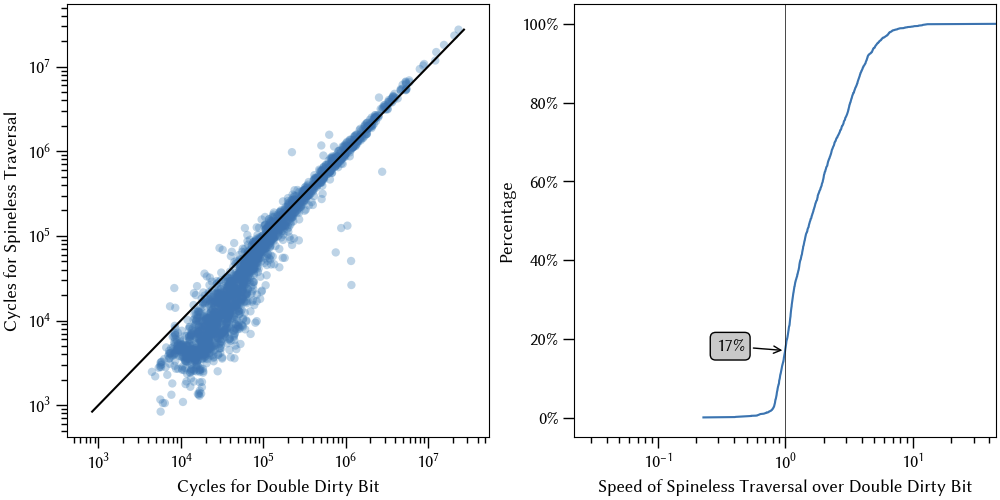
\includegraphics[scale=0.4]{DBPQ.png}
\begin{minipage}[t]{0.48\linewidth}
\caption{
Re-layout time for all \NumFrames frames,
    with Double Dirty Bit time on the $x$ axis
    and Spineless Traversal time on $y$ axis.
The diagonal $x = y$ line shows equal time;
    points below the line are faster with Spineless Traversal
    while points above the line are faster with Double Dirty Bit.
Both axes are in log scale, meaning Spineless Traversal is often
    many faster than Double Dirty Bit.
}
\label{fig:xy}
\end{minipage}\hfill%
\begin{minipage}[t]{0.48\linewidth}
\caption{
  A CDF of the ratio between
    Double Dirty Bit time and Spineless Traversal time
    for each frame.
  The vertical line, at $10^0 = 1\times$,
    marks where both invalidation algorithms take equal time.
  To the left of the line,
    \PctSlower of frames are slower with Spineless Traversal.
  To the right of the line,
    \PctFaster of frames are faster with Spineless Traversal.
  The geometric mean speedup with Spineless Traversal
    is \MeanSpeedup.}
\label{fig:cdf}
\end{minipage}
\end{figure}

\iffalse
\begin{figure}
\begin{subfigure}{0.5\linewidth}
    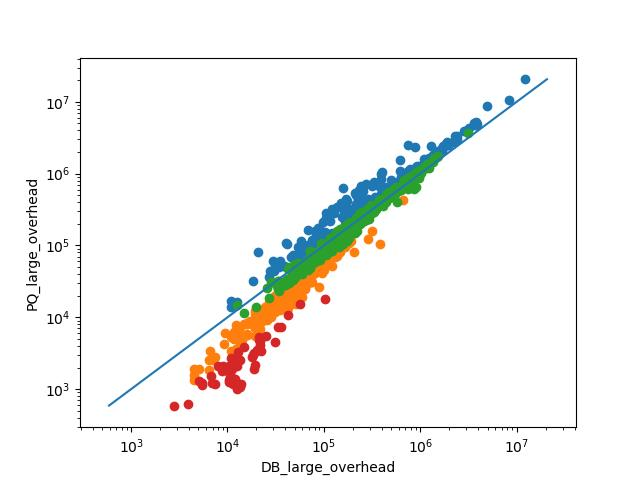
\includegraphics[width=\linewidth]{DBPQLargeOverhead.png}
\end{subfigure}\hfill%
\begin{subfigure}{0.5\linewidth}
    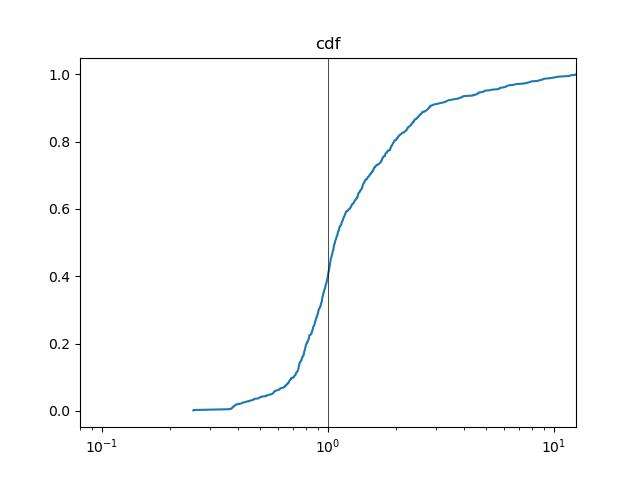
\includegraphics[width=\linewidth]{DBPQLargeCDF.png}
\end{subfigure}
\caption{
The overhead scatter plot and the speedup cdf,
  restricted to frames where more than 1\% of fields
  are recomputed. These points typically represent loading of new contents.}
\label{fig:dbpq-large}
\end{figure}
\fi

\Cref{fig:xy}
  shows our results.
In it, points below the diagonal line
  are frames that are faster with Spineless Traversal,
  while points above the diagonal line
  are frames faster with Double Dirty Bit.
Most frames are below the line:
  only a few deeply-nested nodes are dirtied,
  but Double Dirty Bit makes a huge number of auxiliary accesses,
  which Spineless Traversal avoids.
By contrast, while some points are above the line,
  meaning they are slower with Spineless Traversal,
  the slowdowns are typically much less severe.
The geometric mean is a \MeanSpeedup speedup
  from Spineless Traversal,
  with only \PctSlower of frames rendered slower,
  as shown in \Cref{fig:cdf}.
\Cref{fig:nodes-accessed} shows the reason for this speedup:
  Spineless Traversal simply accesses far fewer nodes
  than Double Dirty Bit.

\Cref{fig:xy,fig:cdf} includes both
  ``overhead'' and ``evaluation'' time.
Evaluation time, as expected, is nearly identical
  between Spinless Traversal and Double Dirty Bit.
Considering overhead alone,
  Spineless Traversal is, for some frames,
  as much as $100\times$ faster than Double Dirty Bit.
For Spineless Traversal,
  overhead time was roughly one third of total runtime,
  while evaluation time was roughly two thirds,
  showing that invalidation overhead is still
  a significant determinant of latency.
Naturally, the slower Double Dirty Bit algorithm
  spends even more time in invalidation overhead.
Breaking overhead time down further for Spineless Traversal
  shows that both the priority queue
  and the order maintenance structure
  contribute to overhead, with different algorithms
  dominating for different benchmarks

A careful inspection of \Cref{fig:xy} shows
  several additional features.
The slowest frames all feature slowdowns.
This is expected: the slowest frames likely represent
  the initial page load or other ``loading'' frames,
  which we necessarily capture in our traces.
While speedups are always better than slow-downs,
  these loading frames likely follow network latency,
  so invalidation time for these frames is less important.
Meanwhile, frames where fewer nodes are invalidated
  are typically those triggered in response to
  an animation or user interaction,
  where latency is most noticeable as ``jank''.
When we restrict the data to only include frames
  where fewer than 1\% of fields are recomputed---%
  the intention being to ignore ``loading'' frames---%
  the geometric mean speedup is larger,
  at \MeanSpeedupSmall,
  and a smaller fraction of frames (\PctSlowerSmall) suffer slowdowns.
Spineless Traversal is also faster outside this subset,
  likely because the 1\% threshold is an imprecise heuristic,
  but the larger speedup 
  in this latency-critical subset is indicative.

\begin{figure}
\begin{minipage}{.59\linewidth}%
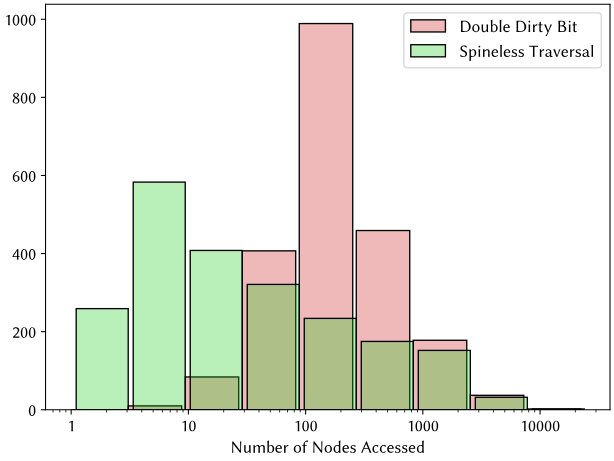
\includegraphics[width=\linewidth]{DBPQHist.png}%
\caption{Histograms of Number of Nodes Accessed by Double Dirty Bit and Spineless Traversal. Double Dirty Bit access much more nodes compare to Spineless Traversal, so the latter cause much fewer cache misses.}
\label{fig:nodes-accessed}
\end{minipage}\hfill%
\begin{minipage}{.39\linewidth}%
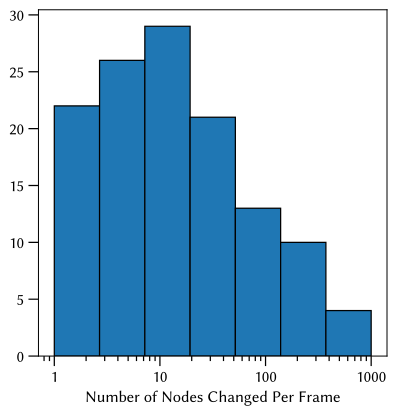
\includegraphics[width=\linewidth]{CaseStudy.png}
\caption{The numbers of Twitter nodes changed externally for each frame. Most frames modify very few nodes, but a few frames insert/remove large subtrees of up to 787 nodes.}
\label{fig:case-study}
\end{minipage}
\end{figure}

\subsection{Case Study: Twitter}

We now focus specifically
  on our trace of Twitter (now X), a social media platform.
This trace of 125 frames captures the user
  opening the Twitter news feed,
  loading the default number of tweets,
  and scrolling down repeatedly to load more tweets.
Twitter is a large web page,
  and the tree grows to 3\thinspace700 DOM nodes
  with a depth of 53 and a fanout of 128. 
Considering all the frames in aggregate,
  Twitter sees a geometric mean speedup of $1.99\times$ 
  over the Double Dirty Bit algorithm.

Most of the 125 incremental layouts are small,
  dirtying no more than 20 nodes (Figure~\ref{fig:case-study}).
For these frames,
  Double Dirty Bit spends most of its time
  accessing auxiliary nodes.
However, the largest incremental layout
  dirties several hundred nodes.
We now discuss several common kinds of frames
  in the Twitter trace.

\paragraph{Linked Files}
Many layouts are triggered when linked files---%
  JavaScript, CSS, images, and videos---%
  finish loading.
Loading JavaScript might add
  new \texttt{<script>} and \texttt{<style>} elements to the page,
  while loading CSS files can change the CSS properties
  of existing elements.
Loading images and videos, meanwhile,
  changes intrinsic widths and heights
  from 0 to the actual image/video width/height.
Typically only one or a few nodes are dirtied,
  but these nodes are often located deep in the layout tree
  or have many siblings,
  so they have many auxiliary nodes.
Spineless Traversal thus reduces latency for these frames
  by up to $10\times$.
 
\paragraph{Lazy Loading}
Twitter uses a lazy-loading technique
  which first loads a ``shell'' page
  and then gradually adds more and more elements to the shell
  as more content is loaded over the network.
For example, the header bar, side bar, ads, and tweets
  all load separately and require separate incremental layouts.
Scrolling causes yet more content (tweets and ads) to load.
Each of these frames typically involve inserting
  a single large subtree.
Allocating the new nodes' OM objects
  (and possibly rebalancing the OM data structure)
  makes these frames difficult for Spineless Traversal
  despite its bulk insertion optimizations,
  Spineless Traversal is slower than Double Dirty Bit,
  typically by about $2\times$.
That said, the latency
  is partially hidden by the network latency
  of loading the content in the first place,
  so the slowdown here may be less critical
  than for other frames.

\paragraph{Removal}
The Twitter application also occasionally removes
  subtrees that are no longer visible to the user,
  like offscreen content.
Spineless Traversal handles these removals
  much faster than Double Dirty Bit,
  often by $5\times$ or more,
  precisely because these removals
  do not affect what the user sees on the screen.
Twitter also sometimes removes
  individual \texttt{<script>} and \texttt{<style>} elements
  that don't affect the page;
  here Spineless Traversal's speedup
  is smaller, approximately $2\times$,
  as multiple elements are removed at once,
  amortizing the auxiliary accesses in Double Dirty Bit. 

Moreover,
  some frames mix file loading, lazy loading, and removals,
  probably at the whim of the task scheduler.
Often many images load in at once.
In this case the time taken for Spineless Traversal 
  basically sums over the time for each individual change,
  while Double Dirty Bit can amortize the cost
  of traversing auxiliary nodes.
These frames are often small,
  so Spineless Traversal's speed-ups are still substantial,
  but probably smaller than if each modification
  was laid out in its own frame.

\section{Related Work}
Incremental Evaluation of interactive programs have yield a long line of fruitful research, dating back to the 1980s (\citet{TR}), and including work such as \cite{yufeng-2}, \cite{SAC}. OTOH, the industry had developed their own solution, the Double Dirty Bit algorithm, to fulfill their latency need.
\section{Conclusion}
%\bibliographystyle{acm}
\bibliographystyle{ACM-Reference-Format}
\bibliography{main}
\end{document}
